\documentclass[10pt]{article}

% The theorem system and user-defined commands
%% implication commands
\newcommand{\R}{\Rightarrow}
\newcommand{\LL}{\Leftarrow}

%% polynomial commands
\newcommand{\polyr}{\mathcal{P}(\mathbb{R})}
\newcommand{\polyn}[1]{\mathcal{P}_{#1}(\mathbb{R})}
\newcommand{\polync}[1]{\mathcal{P}_{#1}(\mathbb{C})}


%% probability commands
\newcommand{\EXP}[1]{\mathbb{E}\left[#1\right]}
\newcommand{\Var}[1]{\text{Var}\left(#1 \right)}
\newcommand{\Bnm}[2]{\text{Binom}\left(#1,#2\right)}
\newcommand{\indy}[1]{\bm{1}_{\{#1\}}}
%% Misc.

\newcommand{\tnl}[1]{\label{eq:#1}\tag{#1}}


%% Number set commands
\newcommand{\RR}{\mathbb{R}}
\newcommand{\ZZ}{\mathbb{Z}}
\newcommand{\QQ}{\mathbb{Q}}
\newcommand{\CC}{\mathbb{C}}
\newcommand{\NN}{\mathbb{N}}
\newcommand{\FF}{\mathbb{F}}
\newcommand{\Span}[1]{\text{Span} \left\{#1 \right\}}

%% Vector commands
\newcommand{\V}[1]{\Vec{#1}}
\newcommand{\norm}[1]{\left\lVert #1 \right\rVert}
\newcommand{\proj}[2]{\text{proj}_{\V{#2}}(\V{#1})}
\newcommand{\inp}[2]{ \langle \V{#1} , \V{#2} \rangle }


%% Matrix commands
\newcommand{\trans}[1]{{#1}^\mathsf{T}}
\newcommand{\trace}[1]{\text{tr}(#1)}
\newcommand{\zmatgen}{\mathbf{0}_{m\times n}}
\newcommand{\zmat}{\mathbf{0}}
\newcommand{\rref}[1]{\text{rref}(#1)}
\newcommand{\dete}[1]{\text{det}#1}
\newcommand{\Det}[1]{\text{det}#1}
\newcommand{\tr}[1]{\text{tr}\left(#1\right)}
\newcommand{\Dim}[1]{\text{dim}\left(#1\right)}
\newcommand{\Col}[1]{\text{Col}\left(#1\right)}
\newcommand{\Row}[1]{\text{Row}\left(#1\right)}
\newcommand{\Rank}[1]{\text{Rank}\left(#1\right)}
\newcommand{\Null}[1]{\text{Null}\left(#1\right)}
\newcommand{\ms}[1]{M_{#1}(\RR)}
\newcommand{\Char}[1]{\text{char}(#1)}

%% Function commands
\newcommand{\Img}[1]{\text{Im}\left(#1\right)}
\newcommand{\Ker}[1]{\text{Ker}\left(#1\right)}
\newcommand{\Nullt}[1]{\text{Nullity}\left(#1\right)}


%% Text commands
\newcommand{\rt}[1]{\textcolor{red}{#1}}
\newcommand{\bt}[1]{\textcolor{blue}{#1}}
\newcommand{\ttt}[1]{\texttt{#1}}
\newcommand{\tb}[1]{\textbf{#1}}
\newcommand{\Jup}{\ttt{Jupyter}\textsuperscript{\ttt{TM}}}


%% Right angle tikz definition
\def\MarkRightAngle[size=#1](#2,#3,#4){
  \draw[black,thick] ($(#3)!#1!(#2)$) -- ($($(#3)!#1!(#2)$)!#1!90:(#2)$) -- ($(#3)!#1!(#4)$)
}



\usepackage[left=0.5in,right=1.2in]{geometry} % margin adjustments
\usepackage{graphicx} % to use includegraphics
\usepackage{setspace} % not sure if I need this
\usepackage[inline]{enumitem} % fancy enumerating
\usepackage{float} % fixing figure positions 
\usepackage[dvipsnames]{xcolor} % color text & more
\usepackage[most]{tcolorbox} %colorful boxes
\usepackage{hyperref} % for the hyperreferences
\usepackage[nameinlink]{cleveref} %references
\usepackage{amsmath, amsthm, amssymb, amsfonts} % math tools
\usepackage{pgfplots} %math plots
\usepackage{subcaption} %for subfigures
\usepackage{titlesec} %used to define units
\usepackage{lipsum} % for dummy text in latin 
\usepackage{marginnote} % to write margin notes
%%\usepackage{thmtools} % for custom theorem environments
\usepackage[utf8]{inputenc} % Allows for certain characters
\usepackage{environ} % for new environments??
\usepackage{fancyhdr} % adds the chapter to all pages?
\usepackage{listings}
\usepackage{tikz}
\usepackage{bm}
\usepackage{pdfpages}
\usetikzlibrary{calc}
\usetikzlibrary{angles, quotes}  % for angle marks and labels




%\usepackage{showframe} % shows text frames

\makeatletter
\renewcommand*\env@matrix[1][*\c@MaxMatrixCols c]{%
  \hskip -\arraycolsep
  \let\@ifnextchar\new@ifnextchar
  \array{#1}}
\makeatother

%% Color deinitions
\definecolor{codegreen}{rgb}{0,0.6,0}
\definecolor{codeblue}{rgb}{0,0,0.9}
\definecolor{codered}{rgb}{0.9,0,0}
\definecolor{codegray}{rgb}{0.5,0.5,0.5}
\definecolor{codepurple}{rgb}{0.58,0,0.82}
\definecolor{backcolour}{rgb}{0.95,0.95,0.92}

%% Python Style (for listing package)
\lstdefinestyle{Pythonstyle}{
    language=Python,
    backgroundcolor=\color{backcolour},
    commentstyle=\color{codegreen},
    keywordstyle=\color{codeblue},
    numberstyle=\tiny\color{codegreen},  %% change to bb blue?
    stringstyle=\color{codered},
    basicstyle=\ttfamily\footnotesize,
    breakatwhitespace=false,
    breaklines=true,
    captionpos=b,
    keepspaces=true,
    numbers=left,
    numbersep=5pt,
    showspaces=false,
    showstringspaces=false,
    showtabs=false,
    tabsize=2,
    morekeywords={figure, quiver, xlim, ylim, legend, grid, show},
    literate=*{0}{{{\color{codegreen}0}}}{1}
              {1}{{{\color{codegreen}1}}}{1}
              {2}{{{\color{codegreen}2}}}{1}
              {3}{{{\color{codegreen}3}}}{1}
              {4}{{{\color{codegreen}4}}}{1}
              {5}{{{\color{codegreen}5}}}{1}
              {6}{{{\color{codegreen}6}}}{1}
              {7}{{{\color{codegreen}7}}}{1}
              {8}{{{\color{codegreen}8}}}{1}
              {9}{{{\color{codegreen}9}}}{1}
}


% --- Theorem-like environments (shared counter) ---

\newtcbtheorem[number within=section]{mytheorem}{Theorem}%
{enhanced,
  colback=blue!6,
  colframe=blue!35!black,
  fonttitle=\bfseries,
  coltitle=black,
  boxed title style={colback=blue!18, colframe=blue!35!black},
  attach boxed title to top left={xshift=2mm,yshift=-2mm},
  breakable,
  arc=2mm,
  left=2mm,right=2mm,top=1mm,bottom=1mm,
  label type=mytheorem
}{thm}

\newtcbtheorem[use counter from=mytheorem]{mylemma}{Lemma}%
{enhanced,
  colback=purple!6,
  colframe=purple!35!black,
  fonttitle=\bfseries,
  coltitle=black,
  boxed title style={colback=purple!18, colframe=purple!35!black},
  attach boxed title to top left={xshift=2mm,yshift=-2mm},
  breakable,
  arc=2mm,
  left=2mm,right=2mm,top=1mm,bottom=1mm,
  label type=mylemma
}{lem}

\newtcbtheorem[use counter from=mytheorem]{mycorollary}{Corollary}%
{enhanced,
  colback=orange!6,
  colframe=orange!35!black,
  fonttitle=\bfseries,
  coltitle=black,
  boxed title style={colback=orange!18, colframe=orange!35!black},
  attach boxed title to top left={xshift=2mm,yshift=-2mm},
  breakable,
  arc=2mm,
  left=2mm,right=2mm,top=1mm,bottom=1mm,
  label type=mycorollary
}{cor}

\newtcbtheorem[use counter from=mytheorem]{myexample}{Example}%
{enhanced,
  colback=red!6,
  colframe=red!35!black,
  fonttitle=\bfseries,
  coltitle=black,
  boxed title style={colback=red!18, colframe=red!35!black},
  attach boxed title to top left={xshift=2mm,yshift=-2mm},
  breakable,
  arc=2mm,
  left=2mm,right=2mm,top=1mm,bottom=1mm,
  label type=myexample
}{ex}

\newtcbtheorem[use counter from=mytheorem]{mydefinition}{Definition}%
{enhanced,
  colback=green!6,
  colframe=green!35!black,
  fonttitle=\bfseries,
  coltitle=black,
  boxed title style={colback=green!18, colframe=green!35!black},
  attach boxed title to top left={xshift=2mm,yshift=-2mm},
  breakable,
  arc=2mm,
  left=2mm,right=2mm,top=1mm,bottom=1mm,
  label type=mydefinition
}{def}

% --- cleveref names: use the label types above (NOT tcb@cnt@...) ---

\crefname{mytheorem}{theorem}{theorems}
\Crefname{mytheorem}{Theorem}{Theorems}

\crefname{mylemma}{lemma}{lemmas}
\Crefname{mylemma}{Lemma}{Lemmas}

\crefname{mycorollary}{corollary}{corollaries}
\Crefname{mycorollary}{Corollary}{Corollaries}

\crefname{myexample}{example}{examples}
\Crefname{myexample}{Example}{Examples}

\crefname{mydefinition}{definition}{definitions}
\Crefname{mydefinition}{Definition}{Definitions}


\setstretch{1.2}
\geometry{
    textheight=9in,
    textwidth=6.5in,
    top=1in,
    headheight=12pt,
    headsep=25pt,
    footskip=30pt
}



% ------------------------------------------------------------------------------

\begin{document}

\thispagestyle{fancy}
\fancyhead[l]{\textit{Jose Mu\~{n}oz-Lopez}}
\fancyhead[c]{(MATH 206B: NOTES)}
\fancyhead[r]{}


% ------------------------------------------------------------------------------

\newcommand{\ff}{\mathcal{F}}
\newcommand{\bb}{\mathcal{B}}

\section*{Day 1 $\mid$ Numerical Solutions to Nonlinear Equations} %%01/05/2026
\setcounter{section}{1}
%% theorems : mytheorem, mydefinition, mycorollary, ...

\textbf{Gradescope Code:} 6XJ634 

\subsection{Preliminaries}

\begin{mydefinition}{Nonlinear equation}{nonlineareq}
Let $F:\RR^{d}\to \RR^d$
    \begin{align*}
        F(\bm{x}) &= 0 \\
        f_{1}(...) &=0
    \end{align*} 
\end{mydefinition}


Generally difficult to solve a nonlinear equations.

\begin{itemize}
    \item No \textit{real} solutions $f(x) = x^{2}-4x+5=0$.
    \item Non unique solutions, $f(x)=\sin{x}\cos{x}-1/2=0$, $x=2n\pi +\frac{\pi}{4}$.
\end{itemize}

Numerically solve a nonlinear equations means to approximate a solution.

A \textbf{recipe}: \textit{Consider a nonlinear equation $F(x)=0$, where $F:\RR^{d}\to\RR^{d}$. Find a sequence $\{x_{n}\}_{n\in\NN}$, $x_{n}\to x^{*}$, s.t. $F(x^{*})=0$.}

A \textbf{challenge}: The sequence needs to converge ``fast enough", i.e. time efficiency and accuracy.

\begin{mydefinition}{Big-O and Small-o notation}{O-notation}
    \begin{itemize}
        \item Consider $\{a_{n}\}_{n=1}^{\infty}$ and $\{\beta_{n}\}_{n=1}^{\infty}$. We write $\alpha_n = O(\beta_n)$, if $\exists N, C >0$, s.t. 
        \[
        |\alpha_n|\leq C|\beta_n |, \quad \forall n>N
        \]

        we write $\alpha_n = o(\beta_n)$, if 
        \[
        \frac{|\alpha_n|}{|\beta_n|}\to 0, \quad n\to \infty
        \]
    \item Suppose $f:(0,a)\to \RR$, $g(0,a)\to\RR$. We write $f(h)=O(g(h))$, if $\exists \varepsilon, C >0$ such that,
    \[
    |f(h)| \leq C|g(h)|, \quad\forall 0<h<\varepsilon
    \]

    we write $f(h)=o(g(h))$ if 
    \[
    \frac{|f(h)|}{|g(h)|} \to 0, \; h\to 0
    \]
    \end{itemize}
\end{mydefinition}

Here are some examples of use of the notation.

\begin{myexample}{O Notation w/ Sequences}{o-notation}
    Suppose $\alpha_{n}=\frac{1}{n}$, $\beta_{n}=\frac{2}{n}$, and $\gamma_{n}=\frac{1}{n^{2}}$. 

    \begin{itemize}
        \item Note that $\beta_{n}/\alpha_{n}\leq 2$ thus $\beta_{n}=O(\alpha_{n})$.
        \item Also $\gamma_{n}/ \alpha_{n} = \frac{1}{n}\to 0$ implies that $\gamma_{n}=o(\alpha_{n})$.
    \end{itemize}
\end{myexample}

\begin{mydefinition}{Linear Convergence}{linear-convergence}
    Suppose $\{x_{n}\}_{n=1}^{\infty}$ that converges to $x^{*}$, i.e. $\lim_{n\to \infty}x_{n} = x^{*}$ if $\exists\rho\in[0,1]$, such that

    \[
    \lim_{n\to\infty}\frac{|x_{n+1}-x^*|}{|x_{n}-x^*|}=\rho
    \]

    then,

    \begin{itemize}
        \item $\{x_n\}\to x^*$ \textbf{linearly} if $\rho\in(0,1)$,
        \item $\{x_n\} \to x^*$ \textbf{superlinearly} if $\rho =0$,
        \item $\{x_n\} \to x^*$ \textbf{sublinearly} if $\rho = 1$.
    \end{itemize}
\end{mydefinition}

We have the following examples.

\begin{myexample}{}{linearity}
    \begin{enumerate}[label = (\roman*)]
        \item $a_n = 1+2^{2-n}$. We note that $a_{n}\to 1$. We check linearity.

        \begin{align*}
            \frac{|a_{n+1}-x^*|}{|a_{n}-a^*|} &= \frac{|(1+2^{1-n})-1|}{|(1+2^{2-n})-1|} = \frac{|2/2^{n}|}{|2^{2} / 2^{n}|}\\
            &= \frac{1}{2} \in (0,1)
        \end{align*}

        Thus by definition $a_{n}$ converges linearly to $1$.

        \item Another sequence is $b_{n+1}=2^{-n}b_{n} = \frac{b_{n}}{2^{n}}$. Regardless of what value $b_{0}$ takes on (so long as $b_{0}\in\RR$) then clearly $b_{n}\to 0 = b^{*}$. We check linearity,

        \begin{align*}
            \frac{|2^{-n}x_{n} -0|}{|x_{n}-0|} &= \frac{1}{2^{n}}\to 0 = \rho.
        \end{align*}

        Therefore $b_{n}$ converges to $0$ superlinearly.

        \item Finally consider $c_{n} = \frac{1}{n} \to 0$. Again we check linearity.

        \begin{align*}
            \frac{|1/n+1|}{|1/n|} &= \frac{n}{n+1} \to 1 \implies \rho = 1.
        \end{align*}

        Thus, $c_{n}$ converges to $0$ sublinearly.
        
    \end{enumerate}
\end{myexample}

\begin{mydefinition}{Convergence with order $p$}{order-p-convergence}
    If $\exists p >0, C>0$, such that

    \begin{align*}
        \lim_{n\to\infty} \frac{|x_{n+1}-x^{*}|}{|x_{n}-x^{*}|^{p}} = C
    \end{align*}

    Then $\{x_{n}\}_{n=1}^{\infty}\to x^*$ with order $p$.
\end{mydefinition}

\begin{mylemma}{}{lemma-1}
    If $\{x_{n}\}\to x^*$ with order $p$, the sequence will also converge with order $q$, if $0<q<p$.
\end{mylemma}

\begin{proof}
    \rt{Fill in details of proof}
\end{proof}

\begin{myexample}{The Square Root Algorithm}{square-root-algorithm}
    Consider the sequence $x_{n+1}= \frac{1}{2}\left(x_{n}+\frac{a}{x_{n}}\right)$ for $n=0,1,2,...$ where $a>0$. 
    \begin{enumerate}[label=(\roman*)]
        \item Suppose that $x_{n}\to x^*$, i.e. $\lim_{n\to \infty}x_{n}=x^{*}$. Then it follows that,

        \begin{align*}
            \lim_{n\to\infty}x_{n} &= \lim_{n\to\infty}\frac{1}{2}(x_{n}+\frac{a}{x_n}) \\
            \implies x^* &= \frac{1}{2}x^* + \frac{a}{2x^{*}} \\
            \implies (x^{*})^{2} &= \frac{1}{2}(x^{*})^{2} + \frac{a}{2} \\
            \implies (x^{*})^{2} &= a \\
            \implies x^{*} &= \sqrt{a}
        \end{align*}

        \item Now we WTS $x_{n}\to x^*$ with order 2. 

        \begin{align*}
            \frac{|x_{n+1}-x^*|}{|x_{n}-x^*|} &= \frac{|\frac{1}{2}(x_{n}+\frac{a}{x_n})-x^*|}{|x_{n}-x^*|^2} \\
            &= \frac{\frac{1}{2} (x_{n}+\frac{a}{x_n})-\sqrt{a} }{(x_{n}-\sqrt{a})^2} \\
            &= \frac{1}{2} \frac{\left( \sqrt{x_n} -\frac{\sqrt{a}}{\sqrt{x_n}}\right)^2}{(\sqrt{x_n}-\sqrt{a})^2} \\
            &= \frac{1}{2x_{n}} \frac{(x_{n}-\sqrt{a})^2}{(x_n -\sqrt{a})^2} =\frac{1}{2x_{n}}\xrightarrow{n\to\infty} \frac{1}{2\sqrt{a}}=C
        \end{align*}

        Therefore $x_{n}\to \sqrt{a}$ with order 2.
    \end{enumerate}
\end{myexample}


\subsection{Iterative Methods}

One utility of iterative methods is finding roots of functions. Consider for example a function $F(x)$ and our goal is finding a sequence $\{x_{n}\}\to x^*$ such that $F(x^*)=0$. We will explore the \textit{Bisection method} and \textit{Fixed-Point iteration / Newton's Method}.

\begin{mytheorem}{Intermediate Value Theorem (IVT)}{IVT}
    If $f\in C([a,b])$, and $f(a)<k<f(b)$, then $\exists p\in [a,b]$ such that $f(p)=k$.
\end{mytheorem}

\begin{mycorollary}{IVT}{ivt}
    If $f\in C([a,b])$ and $f(a)f(b)<0$, then there exists $p\in [a,b]$ such that $f(p)=0$. \rt{Using this assumption and finding $p$, the root, is the goal of the bisection algorithm.}
\end{mycorollary}

\begin{figure}[H]
    \centering
    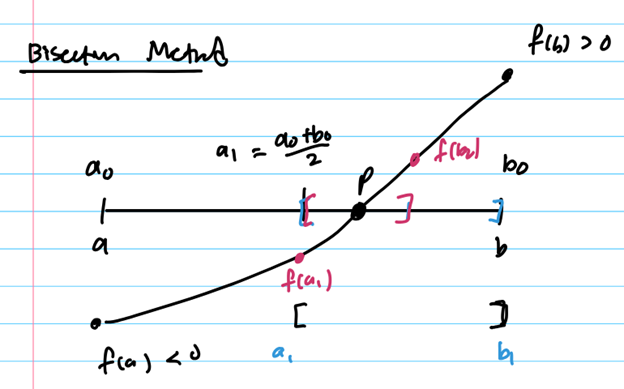
\includegraphics[width=0.7\linewidth]{Images/BisectionAlg.png}
    \caption{Bisection Algorithm Intuition Image}
    \label{fig:BisecAlg}
\end{figure}

Note that $[a_{0}, b_0 ] \supset [a_1, a_2] \supset \cdots$. Note that $\bigcap_{i}[a_{i}, b_i]$ is nonempty. In fact $\lim_{n\to\infty}\bigcap_{i}[a_{i}, b_i] = p$ the root of our continuous function. At each step $a_{n+1}$ becomes the midpoint of $a_{n}$ and $b_n$ while $b_{n+1}=b_{n}$ or $b_{n+1}$ becomes the midpoint and $a_{n+1}=a_{n}$.



\section*{Day 2 $\mid$ Iterative Methods Continued}
\setcounter{section}{2}
\subsection{An Aside On Coding Structure}

\begin{lstlisting}[style = Pythonstyle]
    General Code Set-up

    %Initialization
    parameters; #Define all numbers as parameters.
    structures; #Includes all definitions and functions

    %Main
    for i in 1:nsteps
        %update #For large problem disect -> write in comments -> code
                #skeleton and slowly flesh out
        %visualize / save data #visualization helps with debugging!

    end
    #save data
\end{lstlisting}

\subsection{More Preliminaries}

\begin{mydefinition}{Absolute Error \& Relative Error}{absolute-and-relative-error}
    Suppose that $\{x_{n}\}_{n=1}^{\infty}\to x^*$. The \textbf{absolute error} $x^*$ and the approximation $x_{k}$ us the error given by $|x_{k}-x^{*}|$. If $x^* \neq 0$, then the \textbf{relative error} is $\frac{|x_{k}-x^*|}{|x_k |}$. 
\end{mydefinition}

\subsection{Bisection Algorithm}

We return to the bisection algorithm we described last class. We have the following theorem.

\begin{mytheorem}{Bisection Algorithm Theorem}{bisection-algorithm}
    Suppose $f\in C([a,b])$ and $f(a)f(b)<0$. Then the bisection algorithm generates $\{[a_n, b_n]\}_{n=0}^{\infty}$ and the associated midpoints $x_{n} = \frac{a_{n}+b_n}{2}$. 

    \begin{enumerate}[label = (\roman*)]
        \item The sequences $\{a_n\}$, $\{b_n\}$, and $\{x_n\}$ all converge to $x^*\in [a,b]$,
        \item $f(x^*)=0$,
        \item and the absolute error is bounded in the following manner,
        \[
        |x_k - x^*| \leq \frac{1}{2}(b_{k}-a_{k}) = 2^{-(k+1)}(b-a).
        \]
    \end{enumerate}
\end{mytheorem}

\begin{proof}
    We prove the claims laid out in the Bisection Algorithm Theorem sequentially.
    \begin{itemize}
        \item Note that $\{a_n\}$ is monotonically increasing and has an upper bound $b$. Thus $a_{n}$ is guaranteed to converge by the Monotone Convergence Theorem. Let $A:=\lim_{n\to\infty}a_{n}$. Similarly $\{b_{n}\}$ is bounded below by $a$ and is monotone decreasing, thus this sequence too converges. Let $B:=\lim_{n\to\infty}b_{n}$.

        \begin{align*}
            |A-B| &= |\lim_{n\to \infty}a_{n} -\lim_{n\to \infty}b_{n} | \leq \lim_{n\to\infty}|a_n  - b_n| \\
            &= \lim_{n\to\infty}\frac{1}{2}|a_{n-1}-b_{n-1}| = \cdots =\lim_{n\to\infty}\frac{1}{2^{2}}|a_{0}-b_{0}| \\
            &= \lim_{n\to\infty}\frac{1}{2^{n}}|b-a| = 0.
        \end{align*}

        Therefore $A=B$. Let $x^* := A=B$. Finally since $a_{n}\leq x_{n}\leq b_{n}$ then by the squeeze theorem we have that $x_{n}\to x^*$.

        \item From assumptions from the bisection algorithm we have that $f(a)f(b)<0$, $f$ is continuous, and $f(a_{n})f(b_n)\leq 0$ for all $n$. Thus it follows that,

        \[
        \lim_{n\to\infty}f(a_n)f(b_n) = f^{2}(x^*) \leq 0 \implies f(x^{*}) = 0.
        \]

        \item Finally we note that $x^*\in \bigcap_{n=0}^{\infty}[a_{n}, b_{n}]$. Consider some approximation of $x^*$, namely $x_{n}$. Note $x_{n}\in [a_{n}, b_{n}]\cap [a_{n+1}, b_{n+1}]$, this is because the midpoint of $[a_n, b_n]$, which is $x_n$, will be either $a_{n+1}$ or $b_{n+1}$ by the bisection algorithm. This allows us to bound our absolute error after $n$ steps of the bisection algorithm. Namely we have,

        \begin{align*}
            |x_{n}-x^*| &\leq |b_{n+1}-a_{n+1}| = \frac{1}{2}|b_{n}-a_{n}|=\cdots =\frac{1}{2^{n+1}}|b_{0}-a_0 | = \frac{1}{2^{n+1}}|b-a|
        \end{align*}
    \end{itemize}
\end{proof}

This end our discussion on the bisection algorithm. There are some obvious limitations to the algorithm. For example imagine a function that is mostly positive and has a sharp drop to below the $x$ axis. In such a case the condition on the interval $[a,b]$ would be difficult to meet in practice. There is some inherent intuition one would need about a functions root to pick the proper interval. For example consider a function $f(x)=x(x-1)(x+1)$ and the interval $[-2,3]$. Following the bisection algorithm would yield the single root $x=1$. One would have to construct other intervals to get the remaining roots.


\subsection{Fixed-Point Problems: An Introduction}

\begin{mydefinition}{Fixed-Point Problem}{fixed-point-problem}
    The value $x^*$ is a fixed point for a given function $g$ if $g(x^*)=x^*$. The problem of finding $x^*$ such that $g(x^*)=x^{*}$ is called a \textbf{fixed-point problem}. 
\end{mydefinition}

\begin{myexample}{}{fixed-points}
    Consider the function $g(x)=x^{2}-2$, note that it has the following fixed points,

    \begin{align*}
        g(-1)&=-1, \\
        g(2) &=2.
    \end{align*}

    We say $-1,2$ are fixed points of $g$.
\end{myexample}


\textit{Remark: Notice that root finding problems are equivalent to fixed-point problems. That is $f(x)=0 \iff g(x)=x+\alpha f(x)$.}


The following theorem deals with fixed points and contraction mappings. The short of it is that a contraction mapping (that is continuous) is guaranteed to have a fixed point and further assumptions guarantee uniqueness of this fixed point.

\begin{mytheorem}{Fixed Point Contraction Theorems}{fixed-point-contraction}
    \begin{enumerate}
        \item If $g(x)\in C([a,b])$ and $g(x)\in [a,b]$ for any $x\in [a,b]$ (essentially $g$ is a \textit{contraction mapping} on $[a,b]$), then there exists $x^*\in [a,b]$ such that $g(x^*)=x^*$.
        \item Additionally, if $g\in C^{1}([a,b])$ and there exists $k\in [0,1)$ such that $|g'(x)|\leq k <1$ for all $x\in (a,b)$ then the fixed point $x^{*}$ is unique.
    \end{enumerate}
\end{mytheorem}

Before providing proofs let's build some intuition. We can do this by visualizing the contraction mapping by creating a square using the intervals $[a,b]$ on both the domain and codomain. We note that $g$ is continuous on the interval and that $\Img{g}\subseteq [a,b]$ (the codomain). Then consider the line created by $f:[a,b]\to[a,b]$ with rule $f(x)=x$. A fixed point of $g$ would translate to an intersection with $f$. 

\begin{figure}[H]
    \centering
    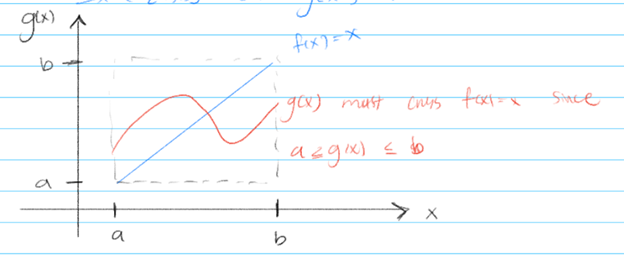
\includegraphics[width=0.7\linewidth]{Images/FixedpointThm.png}
    \caption{Fixed Point Theorem Intuition}
    \label{fig:fixedPointThmIntuition}
\end{figure}

For the second claim of the theorem. The intuition is that for a function to have more than 1 fixed point it would have to have sharper drops and rises within the interval $[a,b]$ but the condition on the derivative of $g$ assures that ``$g(x)$ always changes mildly."


\section*{Day 3 $\mid$ Fixed Point Problems}
\setcounter{section}{3}
We begin by first proving the existence claim of \cref{thm:fixed-point-contraction}.

\begin{proof}
    The trivial case is when $g(a)=a$ or $g(b)=b$, then we have the existence of the fixed point $a$ or $b$. Otherwise note that due to the contraction mapping it must be the case that $g(a)>a$ and $g(b)<b$. Now consider $h(x):= g(x)-x$ and note that $h(a)>0$ and $h(b)<0$, thus since $h\in C([a,b])$ by \cref{cor:ivt} there exists $x^{*}\in [a,b]$ such that $h(x^*)=0$. Which implies that $g(x^{*})-x^{*}=0$ and thus $g(x^*)=x^*$ and we have a fixed point on $[a,b]$. 
\end{proof}

Now we prove the uniqueness of this fixed point under the additional assumption that the contraction mapping has a derivative that has magnitude less than 1 on the interval.

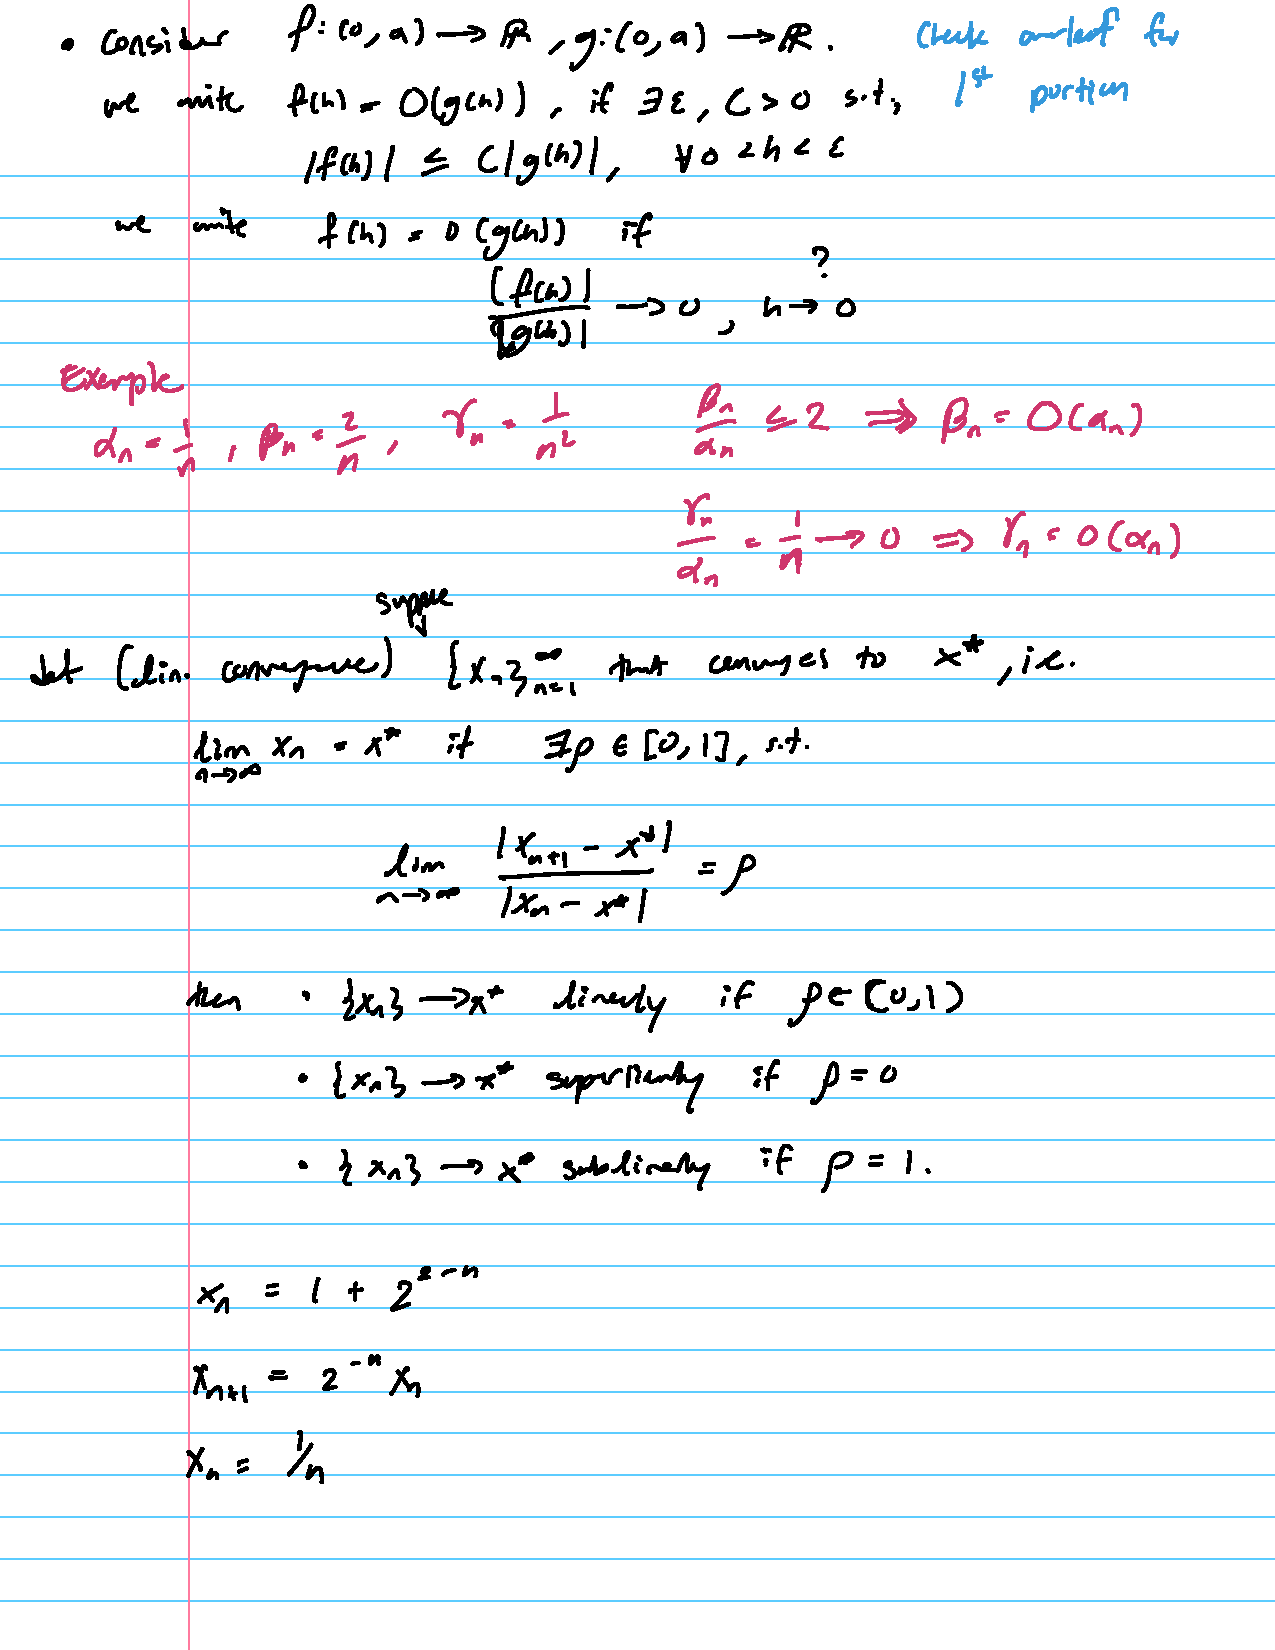
\includepdf[pages=-]{PDFs/NumNote1.pdf} %% 01/05/2026 (M)
                                        %% Prof was out traveling (W)
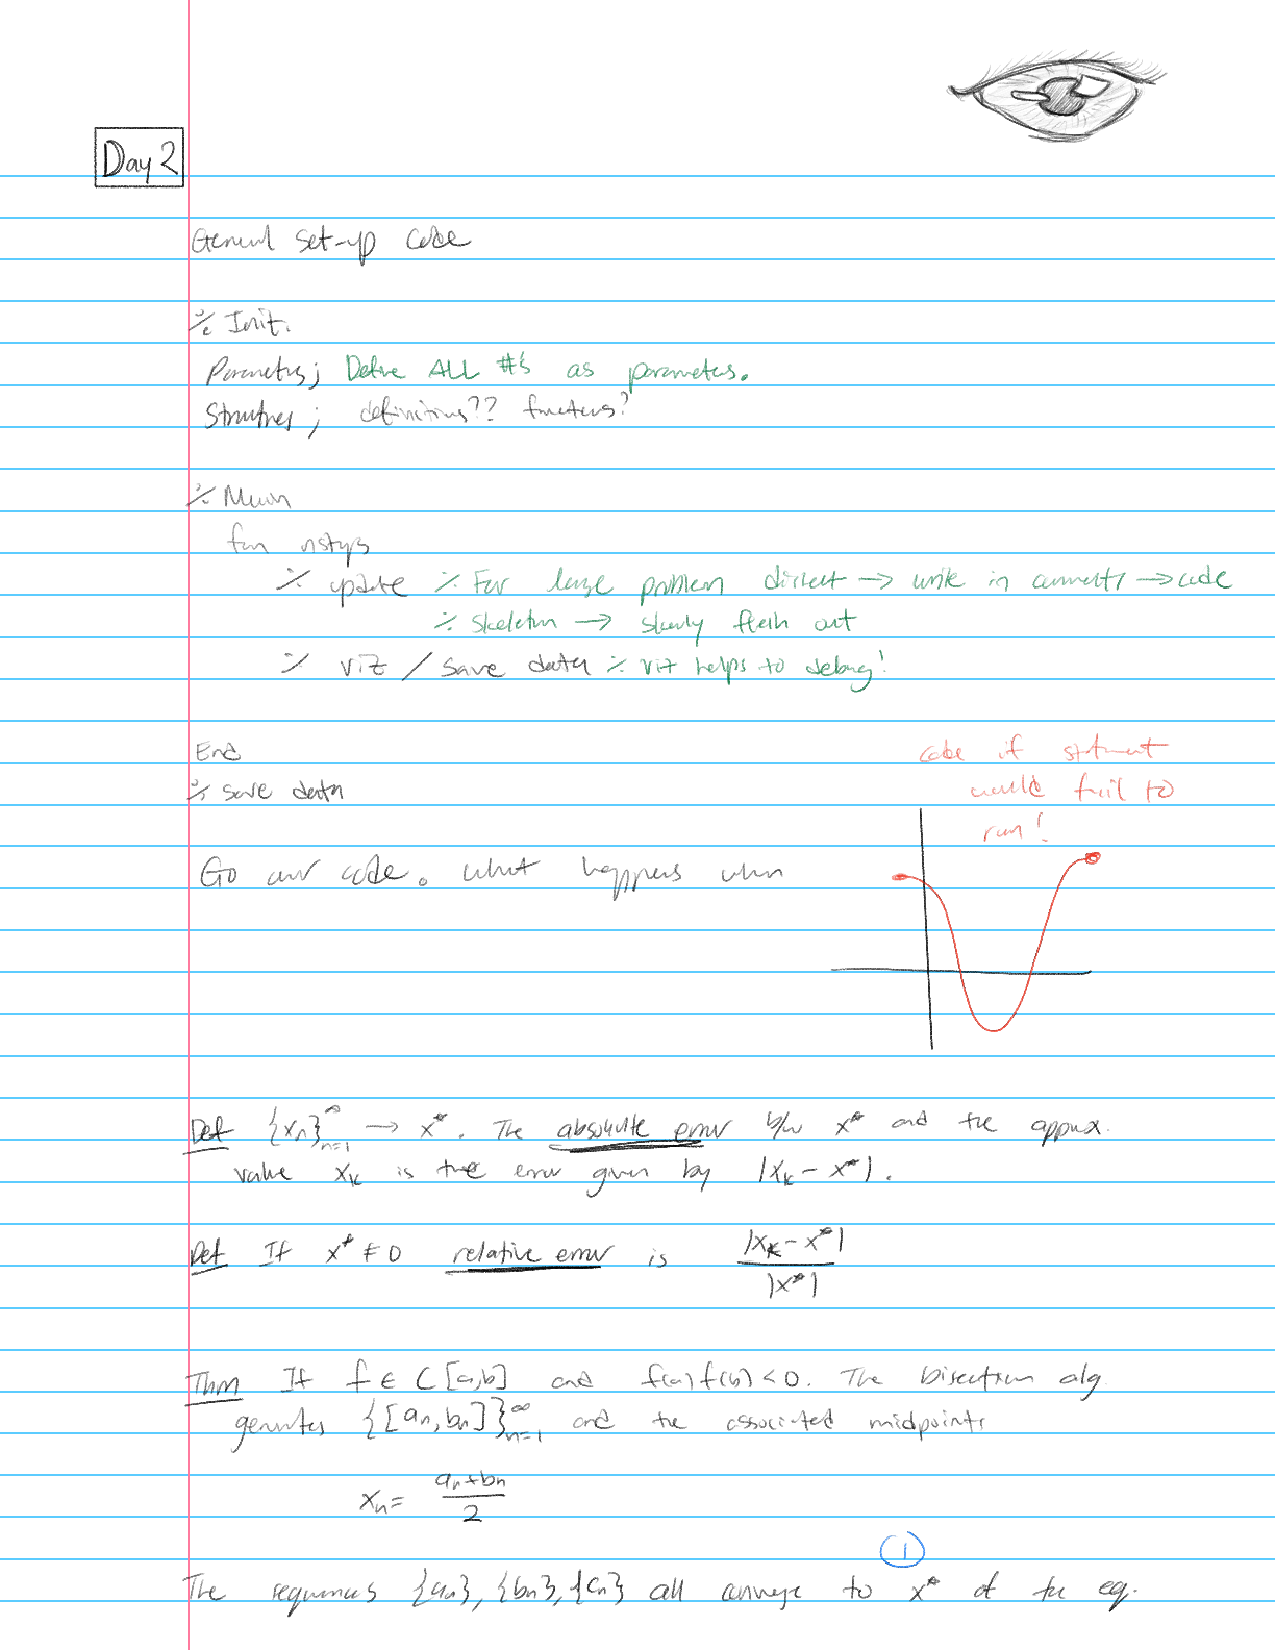
\includepdf[pages=-]{PDFs/NumNote2.pdf} %% 01/12/2026 (M)
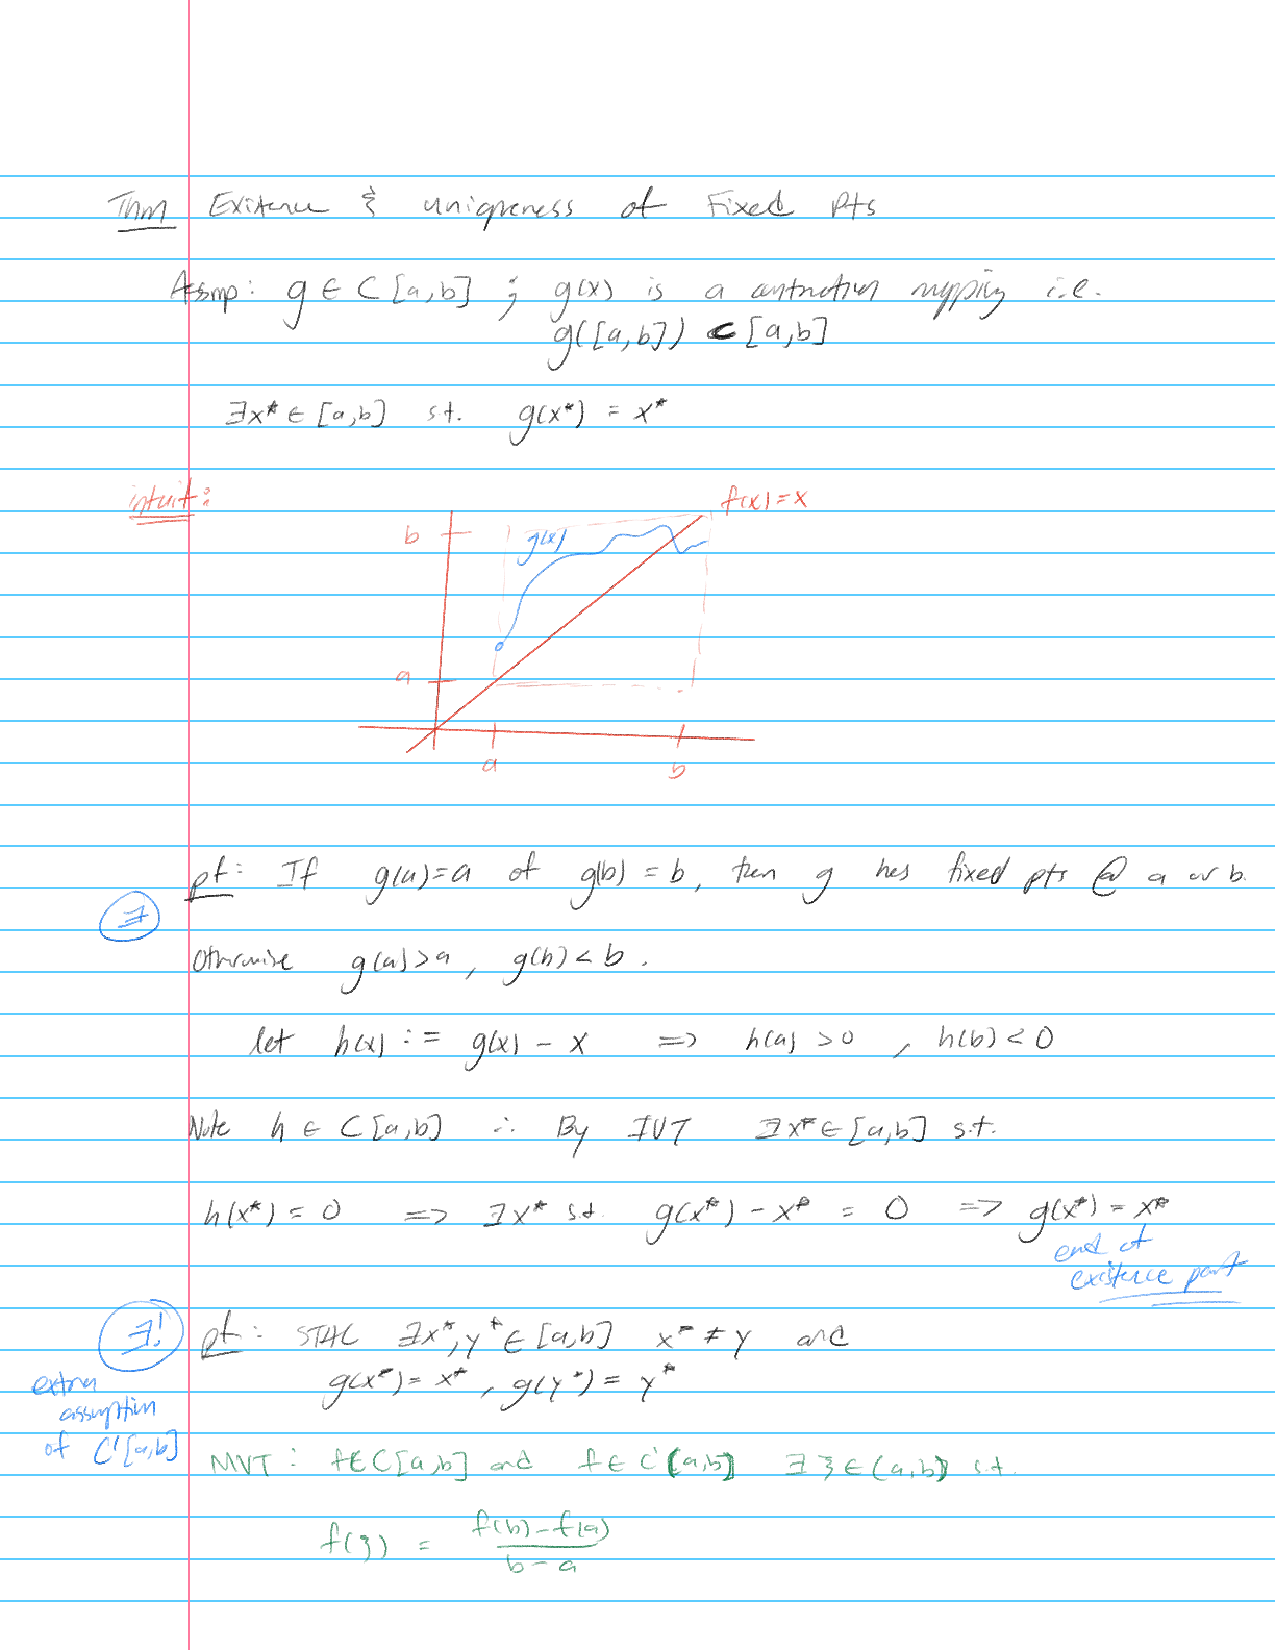
\includepdf[pages=-]{PDFs/NumNote3.pdf} %% 01/14/2026 (W)
                                        %% Holiday (M)
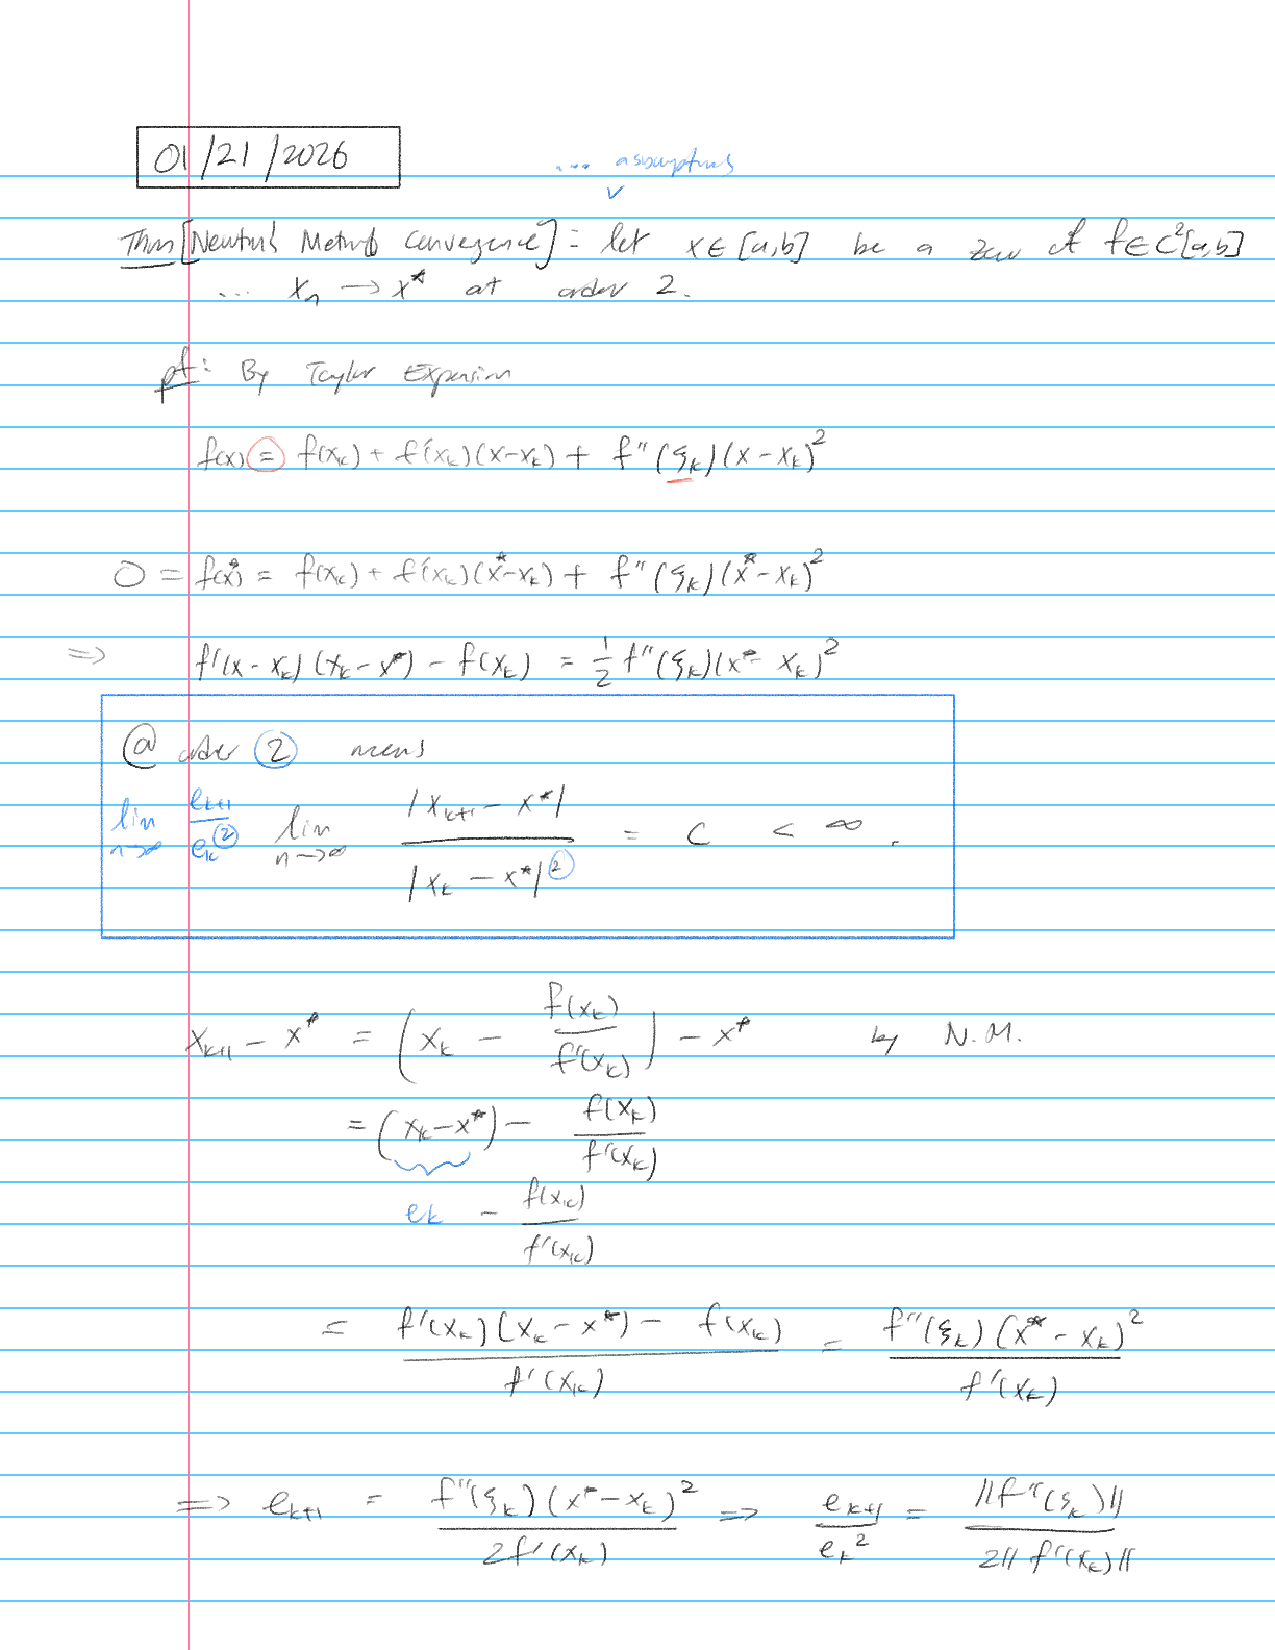
\includepdf[pages=-]{PDFs/NumNote4.pdf} %% 01/21/2026 (W)
%%\includepdf[pages=-]{PDFs/NumNote5.pdf} %% Online Class?? (need notes)
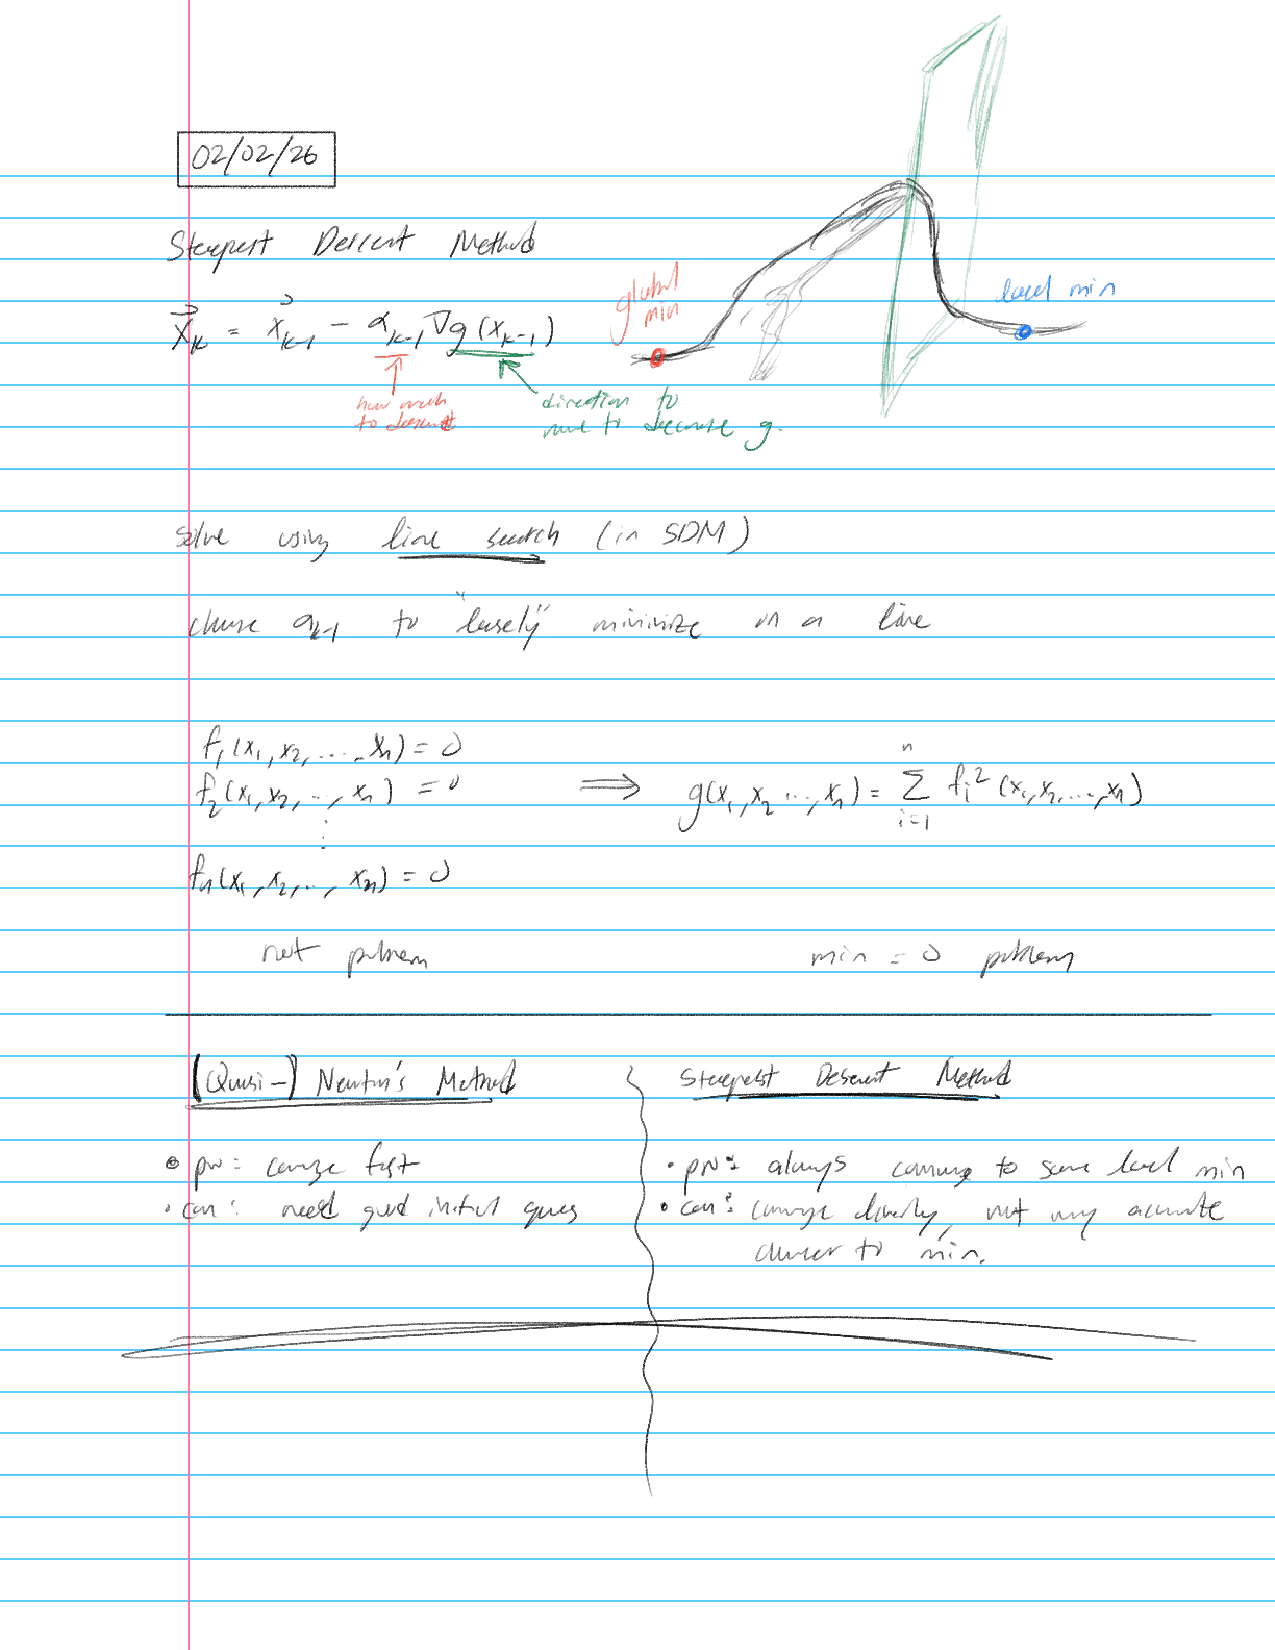
\includepdf[pages=-]{PDFs/NumNote6.pdf} %% 02/02/2026 (M)
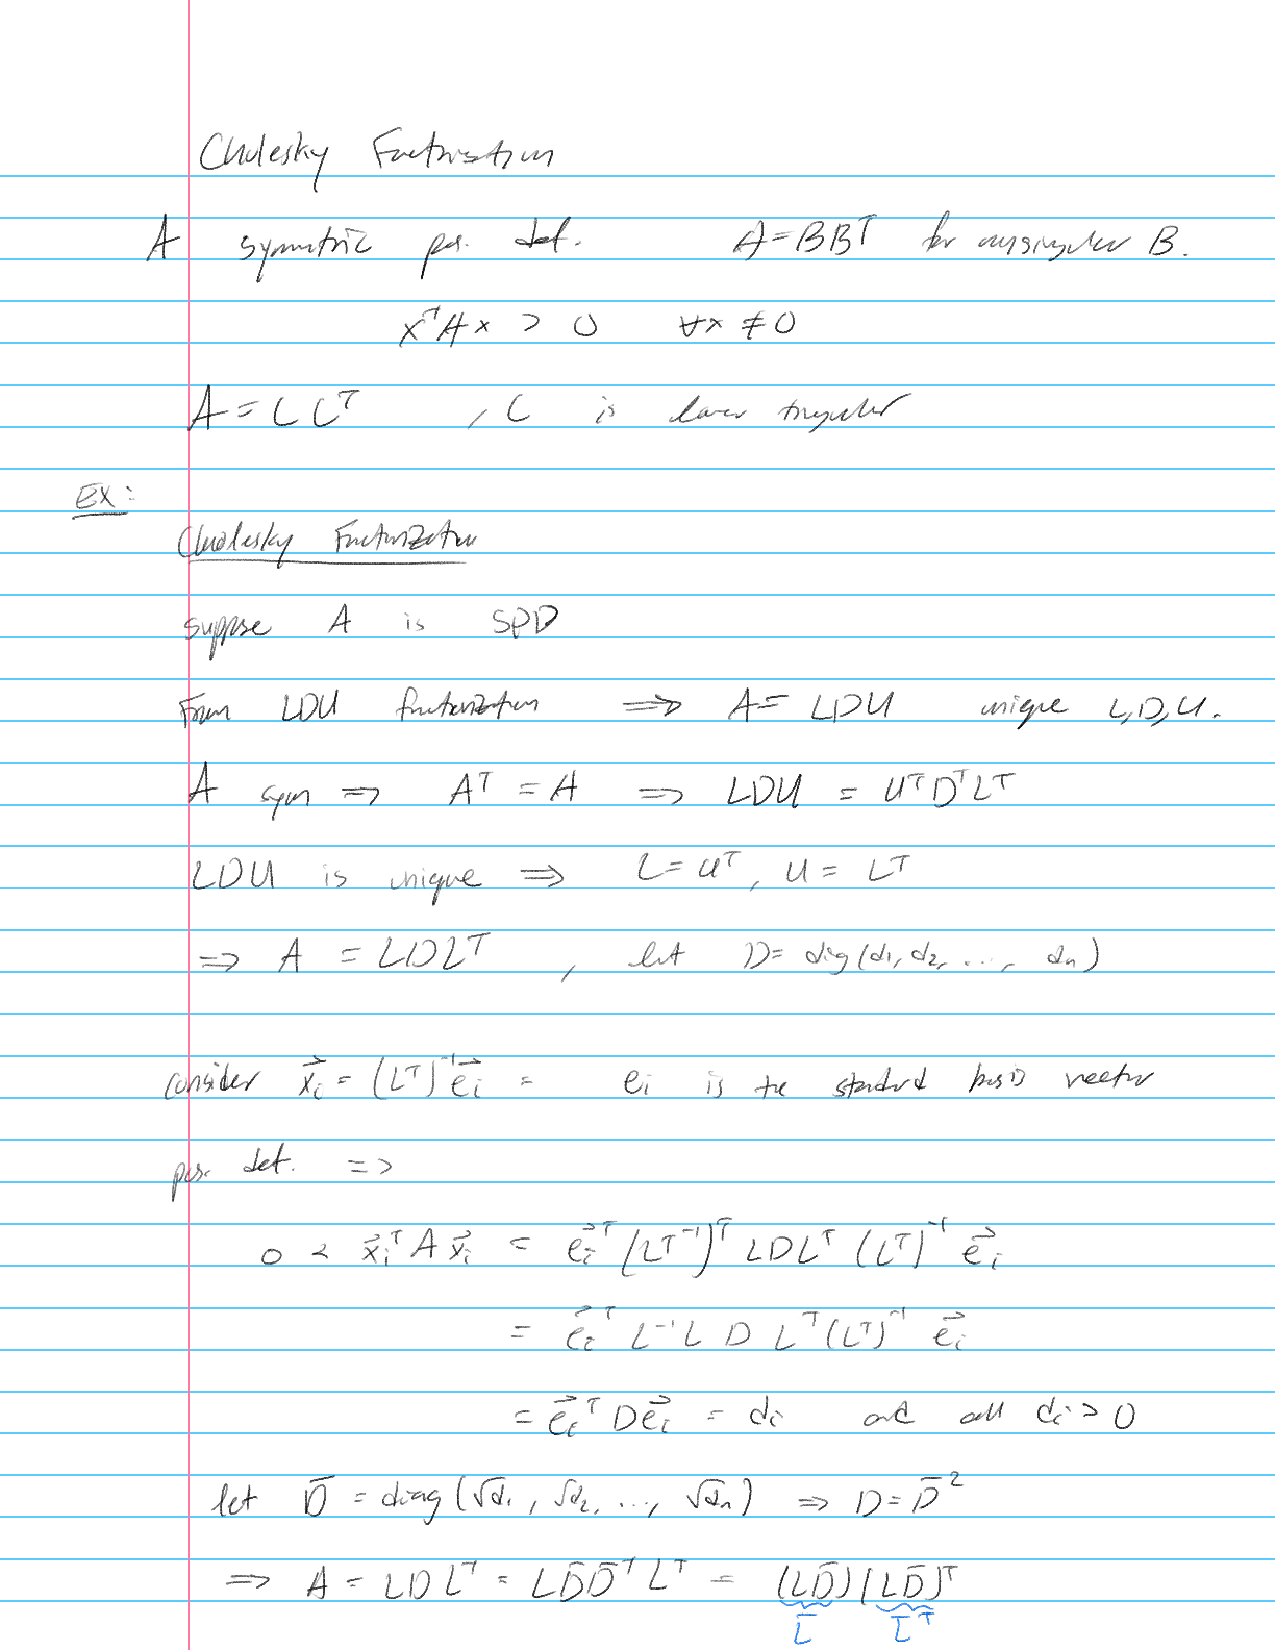
\includepdf[pages=-]{PDFs/NumNote7.pdf} %% 02/04/2026 (W)
\includepdf[pages=-]{PDFs/NumNote8.pdf} %% 02/09/2026 (M)
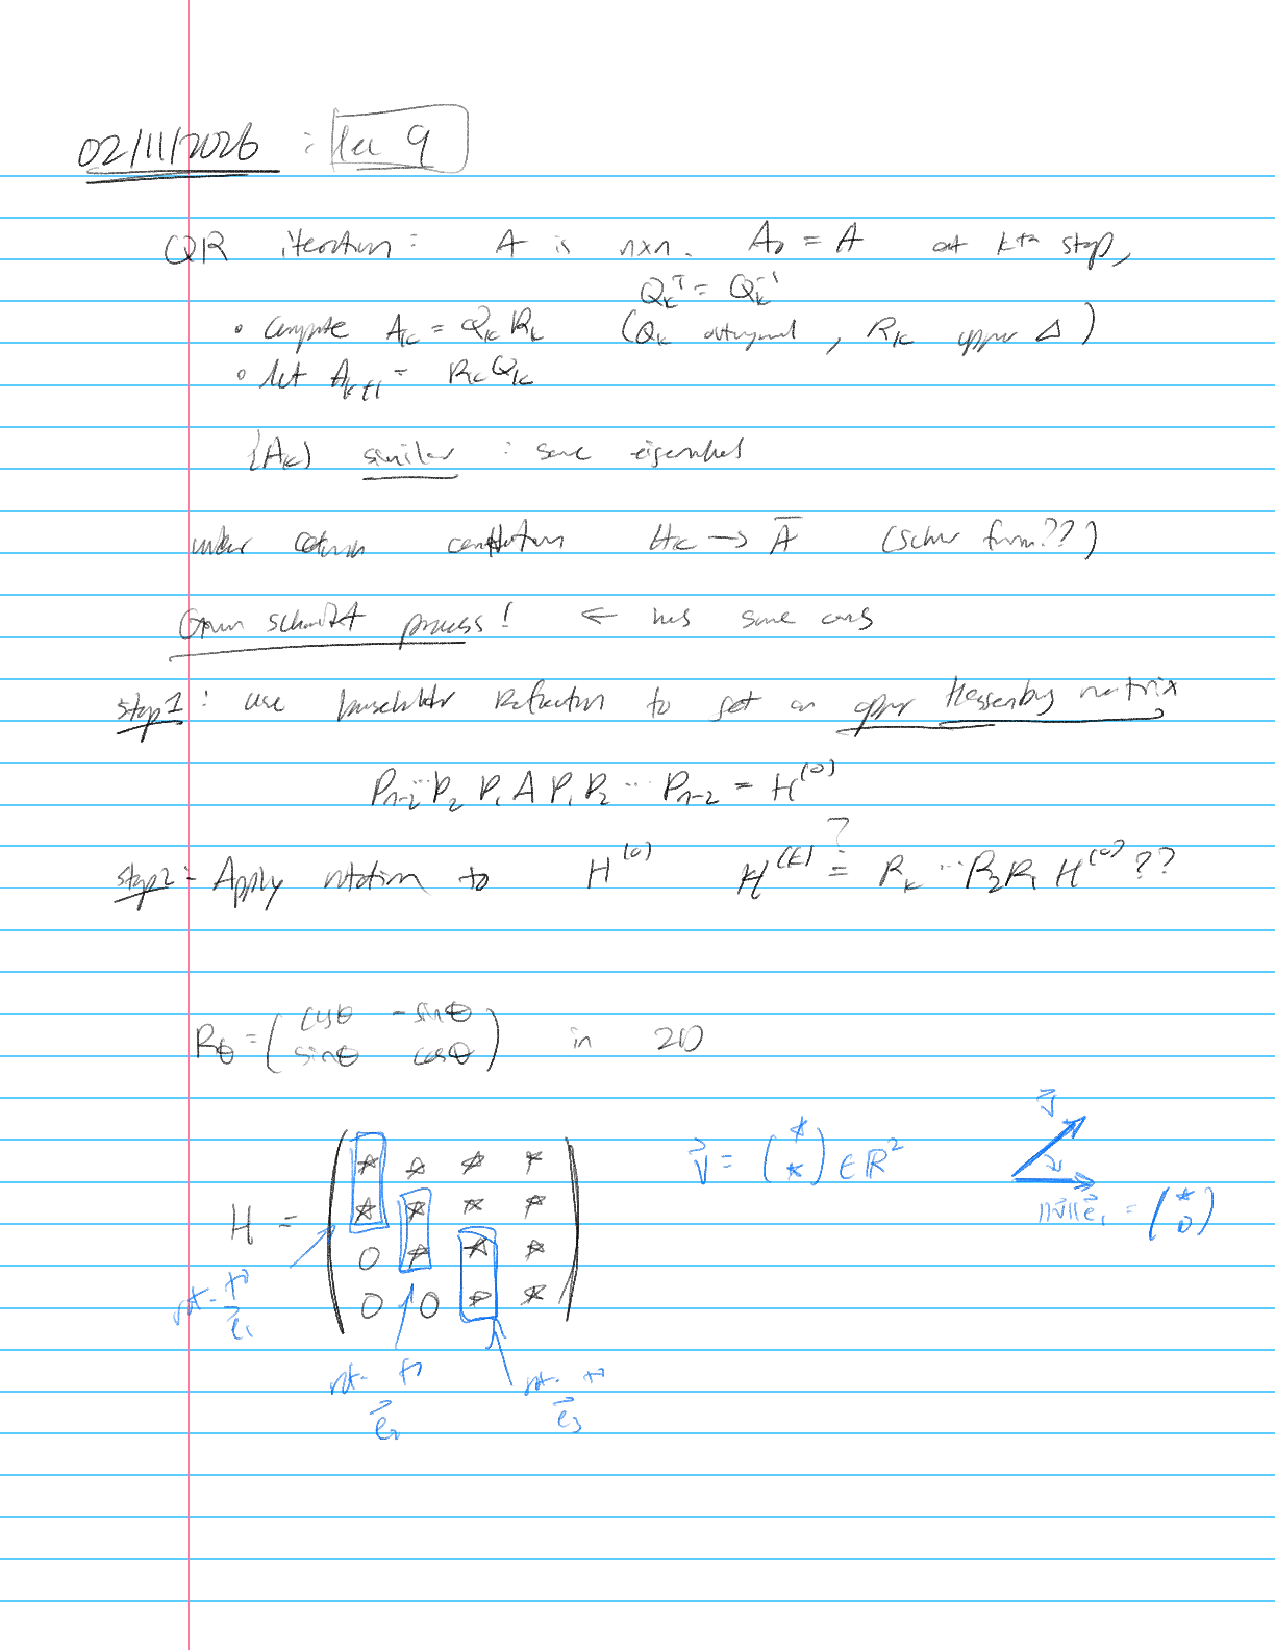
\includepdf[pages=-]{PDFs/NumNote9.pdf} %% 02/11/2026 (W)


\newpage
\section{Day 4 $\mid$ Trying Something}

\newpage
\section{Day 5 $\mid$ Something Again}


\newpage
\section{Day 6 $\mid$ Should Automatically Compile on Git}

\end{document}

